\documentclass{article} % For LaTeX2e
\usepackage{nips13submit_e,times}
\usepackage{hyperref}
\usepackage{url}
\usepackage{graphicx,caption,subcaption,amsmath,amsthm,amssymb}
\newcommand{\bds}[1]{\boldsymbol{#1}}
%\documentstyle[nips13submit_09,times,art10]{article} % For LaTeX 2.09

\title{Formatting Instructions for NIPS 2013}


\author{
David S.~Hippocampus\thanks{ Use footnote for providing further information
about author (webpage, alternative address)---\emph{not} for acknowledging
funding agencies.} \\
Department of Computer Science\\
Cranberry-Lemon University\\
Pittsburgh, PA 15213 \\
\texttt{hippo@cs.cranberry-lemon.edu} \\
\And
Coauthor \\
Affiliation \\
Address \\
\texttt{email} \\
\AND
Coauthor \\
Affiliation \\
Address \\
\texttt{email} \\
\And
Coauthor \\
Affiliation \\
Address \\
\texttt{email} \\
\And
Coauthor \\
Affiliation \\
Address \\
\texttt{email} \\
(if needed)\\
}

% The \author macro works with any number of authors. There are two commands
% used to separate the names and addresses of multiple authors: \And and \AND.
%
% Using \And between authors leaves it to \LaTeX{} to determine where to break
% the lines. Using \AND forces a linebreak at that point. So, if \LaTeX{}
% puts 3 of 4 authors names on the first line, and the last on the second
% line, try using \AND instead of \And before the third author name.

\newcommand{\fix}{\marginpar{FIX}}
\newcommand{\new}{\marginpar{NEW}}

%\nipsfinalcopy % Uncomment for camera-ready version

\begin{document}


\maketitle

\begin{abstract}
...
\end{abstract}

\newpage
\section{Sparse Convex Additive Model}
We consider the following nonparametric regression problem
\begin{equation}\nonumber
          y_{i} = h(\bds{x}_{i}) + \epsilon_{i} = \sum_{d=1}^{p}h_{d}(x_{di}) + \epsilon_{i} \quad (i=1,2,\cdots,n)
\end{equation}
where $\bds{x}_{i}\in\mathbb{R}^{p}$ is the covariate, $y_{i}$ is the response and $\epsilon_{i}$ is the noise. The regression function $h(\cdot)$ is the summation of 
functions $h_{d}(\cdot)$ in each variable dimension. For high-dimensional data, it would be interesting to select the active variables, or equivalently, non-zero $h_{d}(\cdot)$
that contributes to $h(\cdot)$. Without further assumptions, this is the Sparse Additive Model (SpAM). Here we impose an additional constraint that each $h_{d}(\cdot)$ is 
a convex function, which can be represented by its supporting hyperplanes, i.e.,
\begin{equation}\nonumber
      h_{dj} \geq h_{di} + \beta_{di}(x_{dj}-x_{di}) \quad (\forall i,j)
\end{equation}
where $h_{di}\triangleq{}h_{d}(x_{di})$ and $\beta_{di}$ is the subgradient at point $x_{di}$. Hence we can formulate a convex program for the nonparametric regression problem:
\begin{equation}\label{nnp}
     \min_{\bds{h},\bds{\beta}} \ \frac{1}{2n}\sum_{i=1}^{n}(y_{i}-\sum_{d=1}^{p}h_{di})^{2} + \lambda\|\bds{\beta}\|_{\infty,1}  \ \ 
     \textrm{s.t.} \ \sum_{i=1}^{n}h_{di}=0  \  (\forall d), \ \ h_{dj} \geq h_{di} + \beta_{di}(x_{dj}-x_{di}) \  (\forall i,j,d).
\end{equation}
The regularization term $\|\bds{\beta}\|_{\infty,1}$ is used for variable selection, and the equality constraint is an identifiability constraint. 


The program (\ref{nnp}) contains $O(n^{2}p)$ constraints,  which is computationally expensive for large scale problems. Since for scalar convex functions, the subgradient
should increase monotonically, thus we can reformulate (\ref{nnp}) with only $O(np)$ constraints as
\begin{equation}\begin{split}\label{np}
       &\min_{\bds{h},\bds{\beta}} \ \frac{1}{2n}\sum_{i=1}^{n}(y_{i}-\sum_{d=1}^{p}h_{di})^{2} + \lambda\sum_{d=1}^{p}\|\bds{\beta}_{d\cdot}\|_{\infty} \\
       &\ \textrm{s.t.} \ \sum_{i=1}^{n}h_{di}=0, \ h_{d(i+1)} = h_{d(i)} + \beta_{d(i)}(x_{d(i+1)}-x_{d(i)}), \ \beta_{d(i+1)} \geq \beta_{d(i)} \ (\forall d, i)
\end{split}\end{equation}
Here $\{(1),(2),\cdots,(n)\}$ is a reordering of $\{1,2,\cdots,n\}$ such that $x_{d(1)}\leq{}x_{d(2)}\leq\cdots\leq{}x_{d(n)}$
It is easy to verify that the constraints in (\ref{np}) satisfies the constraints in (\ref{nnp}), as
\begin{eqnarray}
  \nonumber \forall j\geq{}i, h_{d(j)}-h_{d(i)} & = \sum\limits_{t=i}^{j-1}(h_{d(t+1)}-h_{d(t)}) = \sum\limits_{t=i}^{j-1}\beta_{d(t)}(x_{d(t+1)}-x_{d(t)})\\ \nonumber
                                                                             & \geq \beta_{d(i)}\sum\limits_{t=i}^{j-1}(x_{d(t+1)}-x_{d(t)}) = \beta_{d(i)}(x_{d(j)}-x_{d(i)}) \\
  \nonumber \forall j<i,         h_{d(j)}-h_{d(i)} &= \sum\limits_{t=j}^{i-1}(h_{d(t)}-h_{d(t+1)}) = \sum\limits_{t=j}^{i-1}\beta_{d(t)}(x_{d(t)}-x_{d(t+1)}) \\ \nonumber
                                                                             & \geq \beta_{d(i)}\sum\limits_{t=j}^{i-1}(x_{d(t)}-x_{d(t+1)}) = \beta_{d(i)}(x_{d(j)}-x_{d(i)}), 
\end{eqnarray}
hence $h_{d(j)}\geq{}h_{d(i)}+\beta_{d(i)}(x_{d(j)}-x_{d(i)}) \ (\forall j)$, which means $\beta_{d(i)}$ is really a subgradient at point $x_{d(i)}$. 
We call the model (\ref{np}) Sparse Convex Additive Model (SCAM). Notice that if we replace $\beta_{d(i+1)} \geq \beta_{d(i)}$ with
$\beta_{d(i+1)}=\beta_{d(i)}$, then it reduces to LASSO.

\section{Optimization}
SPAM in (\ref{np}) is a quadratic program (QP) with $O(np)$ variables and $O(np)$ constraints. 
Directly applying a QP solver would be computationally expensive for relatively large $n$ and $p$. However, notice that variables
in different feature dimensions are only coupled in the term $(y_{i}-\sum_{d=1}^{p}h_{di})^{2}$. Hence we can apply the coordinate descent method,
where in each step we solve the following QP subproblem for $\{\bds{h}_{d\cdot},\bds{\beta}_{d\cdot}\}$ with other variables fixed:
\begin{equation}\begin{split}\nonumber
       &\min_{\bds{h}_{d\cdot},\bds{\beta}_{d\cdot},\gamma_{d}} \ \frac{1}{2n}\sum_{i=1}^{n}((y_{i}-\sum_{r\neq{d}}h_{ri})-h_{di})^{2} + \lambda\gamma_{d} \\
        &\ \textrm{s.t.} \ \sum_{i=1}^{n}h_{di}=0, \ h_{d(i+1)} = h_{d(i)} + \beta_{d(i)}(x_{d(i+1)}-x_{d(i)}), \ \beta_{d(i+1)} \geq \beta_{d(i)}, \ -\gamma_{d}\leq\beta_{d(i)}\leq\gamma_{d} \ (\forall i).
\end{split}\end{equation}
The extra variable $\gamma_{d}$ is introduced to deal with the $\ell_{\infty}$ norm. This QP subproblem involves $O(n)$ variables, $O(n)$ constraints and a sparse structure, 
which can be solved efficiently using optimization packages (e.g., MOSEK).  We cycle through all feature dimensions ($d$) from $1$ to $p$ multiple times until convergence.
Empirically we observe that the algorithm converges in only a few cycles. We also implemented an ADMM solver for (\ref{np}), but found that it is not as efficient as this QP solver.

\newpage
\section{Experiments}
\subsection{Simulations}
Support recovery result goes here ...

\subsection{Boston housing data}
We take the Boston housing data~\cite{?} as a real example. This data set
contains 13 covariates, 506 samples and one response variable, which is
the housing values in suburb of Boston. The data and detailed description
can be found on the UCI website~\cite{?}. 


We first use all $n=506$ samples (with normalization) to train SCAM, using
a set of candidate $\{\lambda^{(t)}\}$ with $\lambda^{(1)}=0$ (no regularization). For each $\lambda^{(t)}$
we obtain a vector $\|\bds{\beta}^{(t)}\|_{\infty}$ of dimension $p=13$. And non-zero
elements in this vector indicates the variables selected using $\lambda^{(t)}$. 
We then plot $\|\bds{\beta}^{(t)}\|_{\infty}$ versus the normalized
norm $\frac{\|\bds{\beta}^{(t)}\|_{\infty,1}}{\|\bds{\beta}^{(1)}\|_{\infty,1}}$ in Figure \ref{SCAM}.
As a comparison we plot the LASSO/LARS result in a similar way in Figure \ref{LASSO}.
From the figure we observe that the first three variables selected by SCAM (corresponding to $\lambda^{(t)}=0.1$) 
and LASSO are the same: LSTAT, RM and PTRATIO, which is consistent with previous findings~\cite{?}.
We then refit SCAM with only these three variables without regularization, and plot the inferred additive
functions in Figure \ref{Convex}. As can be seen, these functions contain clear nonlinear effects which cannot be captured
by LASSO. The shapes of these functions are also in good agreement with those obtained by SpAM~\cite{?}.


Next, in order to quantitatively  study the predictive performance, we run 10 times 5-fold cross validation, following
the same procedure described above (training, variable selection and refitting), and plot the mean and standard
deviation of the predictive MSE in Figure \ref{MSE}. Since for SCAM, the same $\lambda^{(t)}$ may lead to
slightly different number of selected features in different folds and runs, the x-axis (average number of selected features)
for SCAM is not necessarily an integer. Nevertheless, the figure clearly shows that SCAM has a much lower predictive MSE than LASSO. 
We also compare the performance of SCAM with that of Additive Forward Regression (AFR) presented in~\cite{Xi}, and found that they are similar.
The main advantages of SCAM compared with AFR and SpAM are 1) There are no other tuning parameters (such as bandwidth)
besides $\lambda$. 2) SCAM is formulated as a convex program, which guarantees a global optimum.

\begin{figure}[!htpb]
        \centering
        \begin{subfigure}[b]{0.45\textwidth}
                \centering
                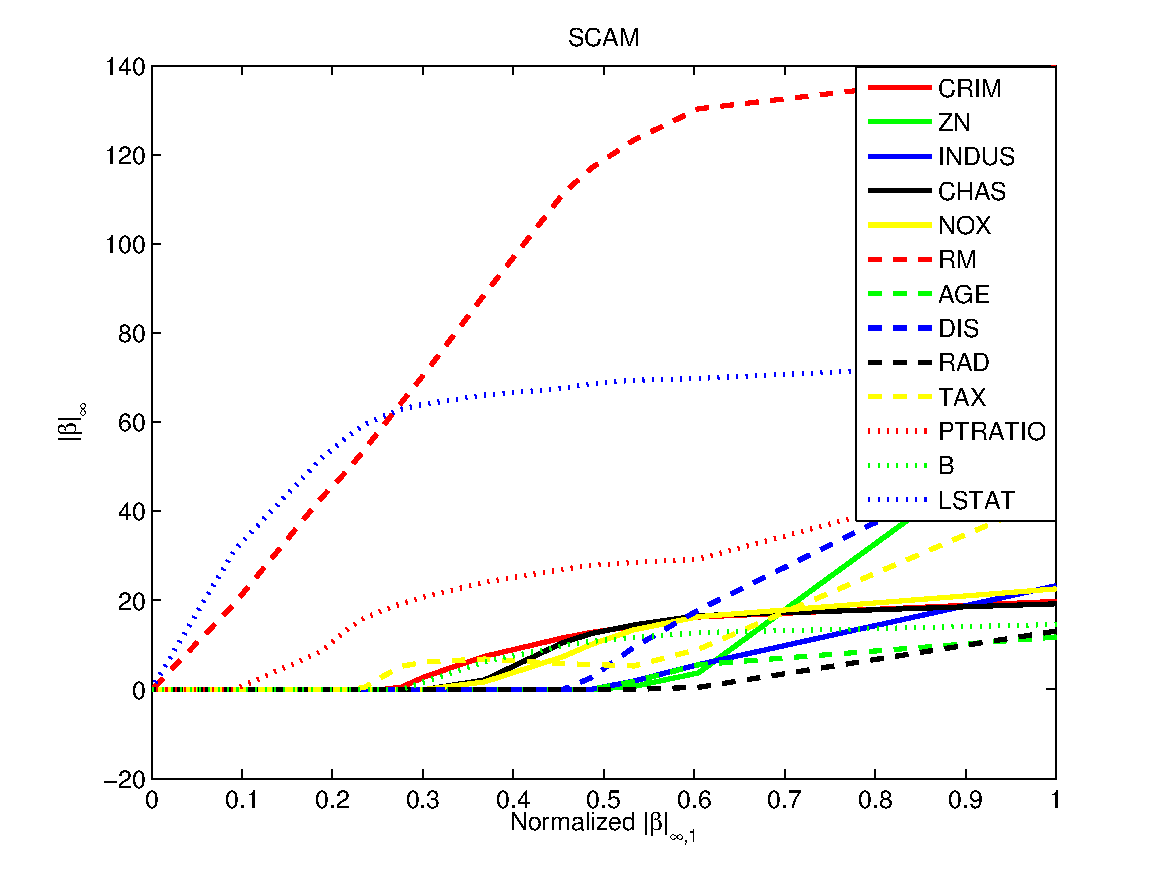
\includegraphics[width=\textwidth]{Additive}
                 \caption{Variable selection result using SCAM.}
                \label{SCAM}
        \end{subfigure}
        \begin{subfigure}[b]{0.45\textwidth}
                \centering
                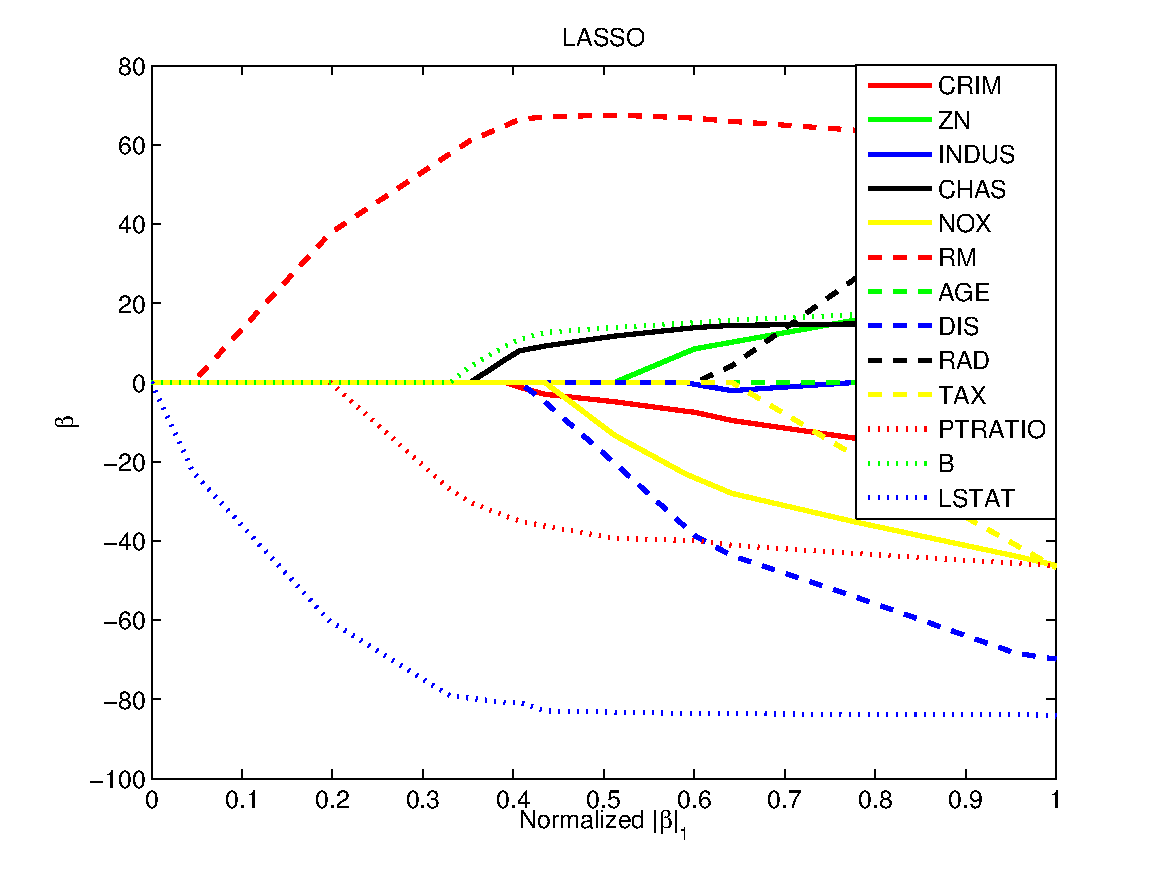
\includegraphics[width=\textwidth]{LASSO}
                \caption{Variable selection result using LASSO.}
                \label{LASSO}
        \end{subfigure}\\
        \begin{subfigure}[b]{0.45\textwidth}
                \centering
                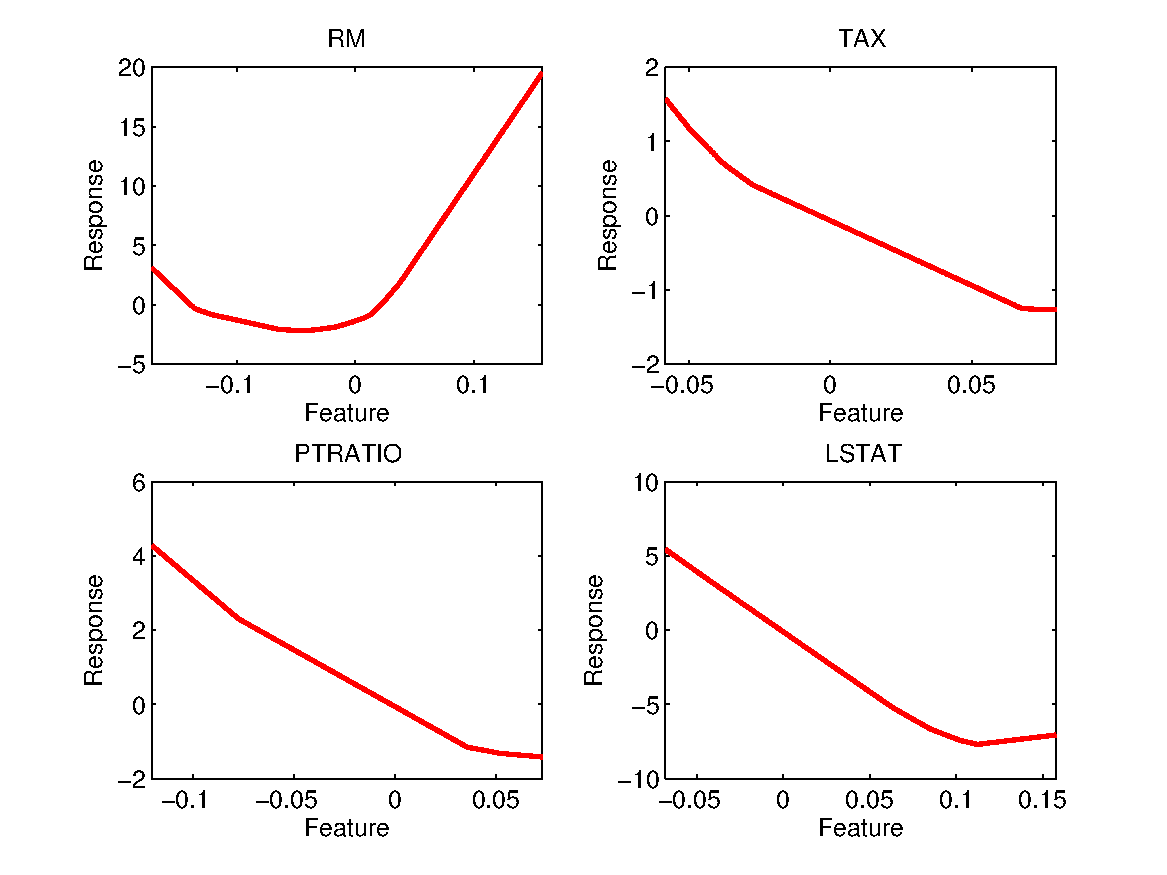
\includegraphics[width=\textwidth]{Convex}
                \caption{Inferred additive convex functions by SCAM.}
                \label{Convex}
        \end{subfigure}
        \begin{subfigure}[b]{0.45\textwidth}
                \centering
                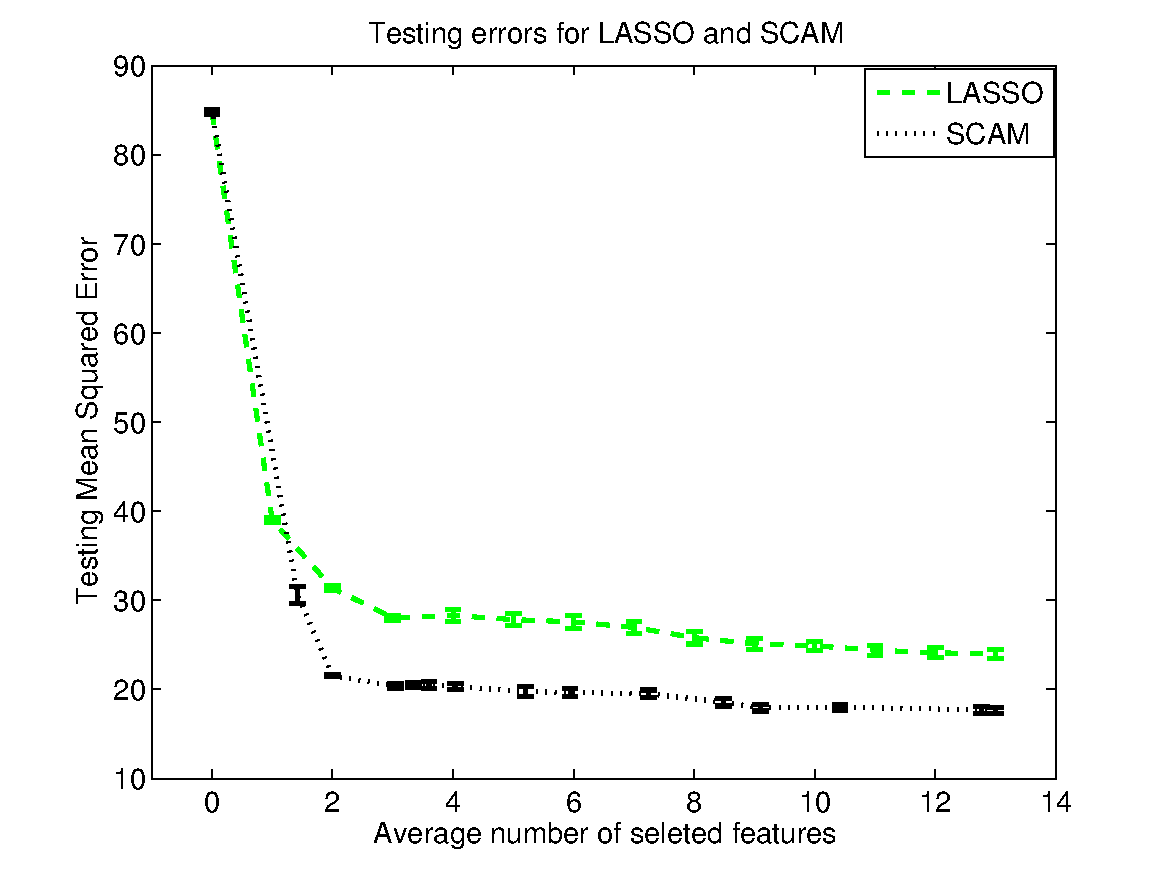
\includegraphics[width=\textwidth]{MSE}
                 \caption{Predictive MSE of SCAM and LASSO.}
                 \label{MSE}
        \end{subfigure}
        \caption{Results on Boston housing data.}\label{Boston}
\end{figure}


\subsubsection*{References}

\end{document}
